\documentclass[twoside, 11pt]{uva-bachelor-thesis}

\usepackage[english]{babel}
%\usepackage{hyperref}
\usepackage{float}
\usepackage{graphicx}

\author{Jan Laan}

\supervisors{Anthony van Inge, Universiteit van Amsterdam}

\signedby{}
\title{Sensor networks with accelerometers for improved spatial location}

\begin{document}

\maketitle

\subsection*{Abstract}
abstract here
\newpage

\tableofcontents

\chapter{Introduction}
GPS based navigation is widely used in various applications and on many devices. However, a huge drawback of the GPS system, is that a GPS receiver needs a direct line of sight to GPS satellites, therefore GPS is very inaccurate indoors. 

This document describes an approach to solve that problem and produce more accurate position data indoors.

\section{Problem Description}
There are multiple methods to determine position with one or more types of sensors. Each method has its own uses and drawbacks. For a set location it is possible to create wireless nodes, transmitting a signal, at known locations, and have receivers pick up that signal. The position is then determined based on the signal picked up from these nodes. \cite{stuvel} This can be done with standard wireless equipment. This method works very well. The drawback of such a method is that the infrastructure needs to be in place, walking into any building is not possible, it will only work for prepared buildings.

Sensors which can be used for determining position by inertial navigation, such as accelerometers, gyroscopes, share the same drawback. They operate on the principle of dead reckoning. Any navigation attempt must start at a known location, after which a new position is determined based on the old location.

\section{Platform}
We will use a number of identical, individual sensor devices with wireless networking capability and a 3-D accelerometer. With these devices we will create a network where these devices can share their, inaccurate, location data. This location data can then be combined  and used to improve the accuracy of ones own location.

This project will be built with the Sun SPOT platform. A SPOT is a small device with a range of sensors and functionalities which can all be accessed by Java libraries. In this project, the most important sensors used are the 3-D accellerometer, and the wireless networking capability of the SPOT. In addition, some LEDs are used for visual feedback.

There are two types of SPOT nodes. The regular node is a wireless device with a battery which can be used for taking measurements from its sensors. The other type is the basestation, which is very similar, but does not have a battery or a sensor board. The basestation is usually attached to a computer with an USB cable. This way, the basestation can communicate wirelessly with the other SPOT nodes and a program on the computer can read and interpret the data the basestation receives.

\chapter{Theory}
This chapter describes the theoretical background of this project. Both data sources used will be described, as well as the method used to combine the data.
\section{Position from accelerometers}
An accelerometer is a sensory device which measures acceleration, the rate of change of speed. This can be defined in $m/s^2$ or in $G$. 1 $G$ is $9.81 m/s^2$, which is equal to the gravitational force of the earth. [??]

The data given by accelerometers can be used to calculate the position of our node, relative to its starting position. The method is as follows: An accelerometer gives the current acceleration in a certain direction, a series of these values can be integrated to find the speed of the node. 

$$S_i = S_{i-1} + A_i \times \delta t$$ 
$S_i$ is the speed of a node at a time $i$ in $m/s$, $A_i$ is its current accelleration in $m/s^2$, and $\delta t$ is the time passed in seconds since the last measurement.
A series of speed measurements can then be integrated again to find the relative location of the node.
$$P_i = P_{i-1} + S_i \times \delta t$$
$P_i$ is the relative position in $m$ at time $i$.


Using three accelerometers along three different axis, the relative position can be determined in three dimensions. Theoretically, this method is ideal. However, in practice this method will usually result in very inaccurate positional data. This is due to several factors.

From the formulas given, we can see that each speed calculation relies on the previous speed calculation. If any calculation result has a small error, due to inaccuracy of the sensor, that error will be added onto by future measurements. This can cause errors to increase over time. The same reasoning applies to the calculation of position. It is dependant on previous calculations in a very similar way. The combination of speed calculations which can be inaccurate, combined with a position calculation which is also inaccurate results in a system with an error that can increase exponentially over time. 

An additional factor is the calculations made to find the speed and position. Because we are using a continuous integration, but an embedded system with limited accuracy, the calculated speed and location are only an approximation. Again, this error will accumulate over time as old values will be used to calculate new speed and location.

As there is no method to 'reset' or know the error obtained by the system, using just accellerometers works fine in theory, buth in practice it is unusable for even a few seconds of position estimation. This will also be demonstrated in the next chapter. More data will be needed to provide a reliable positioning system.
\section{Position from wireless signal strength}
When two wireless devices communicate, a receiver can measure the power of the received signal. This measurement is called the received signal strength indication (RSSI), and is defined in the IEEE 802.15.4 standard. [ref]

RSSI can be used as an indication of distance between two nodes, because the strength of the signal is stronger, the closer the two nodes are together. [SOURCE!!! (experiment?.)] Ideally, one can get a rather exact distance measurement from this value, however there are many pitfalls which make the RSSI measurement unsuitable for location determination on its own.

RSSI only measures distance in one dimension, not location. So, in order to get a relative location, at least 3 other nodes are needed for 2 dimensions, and an additional node for 3 dimensions. So at least five nodes will be needed for this system to work in 3 dimensions.
  [ insert image for clarification ]
  
It is assumed that the strength of the signal emitted by a node is equally strong in all directions. Measurements have shown this is not the case for the Sun SPOT devices.  [imsert img and ref] This results in different values being measured while at the same distance.

Another problem is wireless interference. Other wireless signals, for instance another wireless network, or even a microwave, can interfere and disrupt the signal.
  % needs sources, more explanation on HOW.

Any obstacle such as walls, people, etc. can partially block a wireless signal, so the signal strength can decrease (or even increase under some conditions!)

Lastly, while the method of how and when to read RSSI is defined in the 802.11 standard, what the values actually mean, is not. Different vendors use different scales for RSSI, so these values are not always interchangeable. Because a single platform is used, this is not a problem for us. However, this does mean that their is no defined relation between signal strength and distance. This is a problem that can be overcome.

With all these uncertainties, we can only obtain an approximate distance measurement from the signal strength, which will also only work for one certain device type. Clearly, this is not suitable for providing accurate location data. 

The advantage this method has over reading the accellerometers is that any error does not accumulate over time, it will always stay within limits. [vaag!]


\section{Kalman filters}
As shown in the previous two sections, both accelerometers and wireless signal strength are not suitable for accurate location determination on their own. By combining these two data sources we hope to create a combined system with improved accuracy.

A well known and widely used method for combining multiple data sources is a Kalman filter. A Kalman filter is a recursive algorithm which attempts to eliminate noise from a series of measurements, and to create a more precise estimate of the measured value. There are multiple variants of a Kalman filter, but we will only describe the variant used in this work, a simple discrete Kalman filter.

It can be described as using a two-step process, using the steps "predict" and "correct". At some time, the measurement (position in our case) will be known. Then, in the prediction step, the filter will advance the model in time, and attempt to predict the next measurement value.

$$x_{k+1} = A_kx_k + Bu_k$$

The correction step uses this prediction, and takes a new measurement with which the prediction is corrected. The extent of this correction is based on 

$$$$


obtain new measured data, which will be noisy. In the corrrection step, the previously predicted value will be corrected, based on other data.
\chapter{Implementation}
  \section{Position from accelerometers}
  % how it works, strength and weakness
  As explained before, calculating position from accelerometers alone is very inaccurate. However this is a first step which must be done before it can be improved upon. The formulas described in the previous chapter have been implemented on the SPOT devices. As a test, we have moved a single SPOT node slowly back and forth over a distance of 200 cm and measured its assumed distance from its starting position, which is a combination of all three accellerometers. The results can be seen in the graph below. This test took 57 seconds.

  \begin{figure}[H]
  \centering
  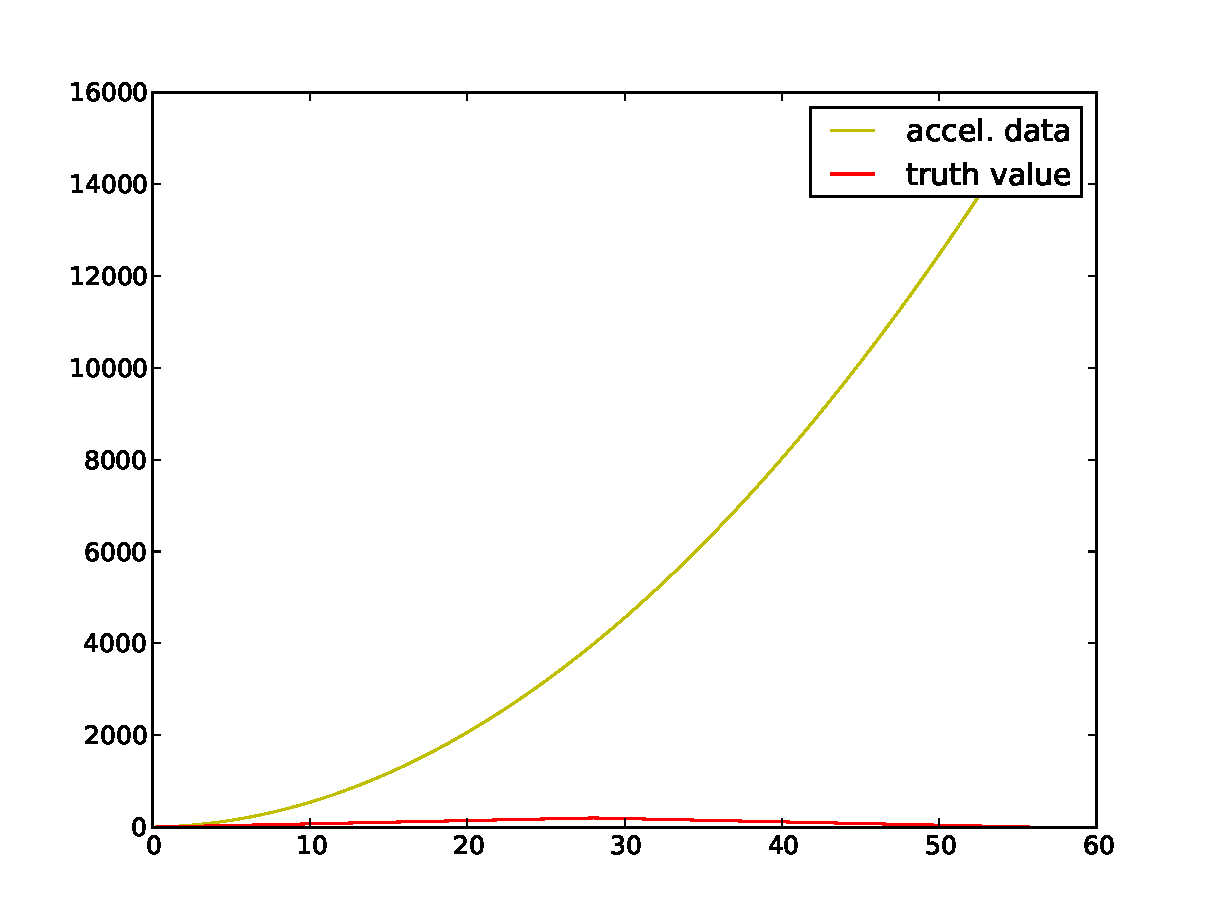
\includegraphics[width=\textwidth]{onlyaccel.pdf}
  \end{figure}
  As can be seen, this is very inaccurate. A small error in the accellerometer values is allowed to increase exponentially. The Ideal result is the red line, which is barely visible above the X-axis. What should be happening is that the measurement goes up to 200 (cm) and then back to 0. Instead is keeps increasing, and ends up at a distance 16000 cm from where it is supposed to, and will keep on increasing. 
  % Image of position increasing exponentially with just accel. data
  
  \section{Distance from radio signal strength}
  % how it works, strength and weakness
  As described in the theory section, we need to map the relation between RSSI and distance for each wireless device. We did this by creating a simple program on a SPOT node, which broadcasts some random data every second. On the basestation side we ran a program which read the RSSI value obtained from the node and saved the values obtained. With these programs, we placed the two devices at a range of set distances from eachother, and performed ten measurements for each distance. This resulted in a scatterplot of a couple hundred measurements. Using functions from the Python module numpy, we fitted a function from these values. 
  \begin{figure}[H]
  \centering
  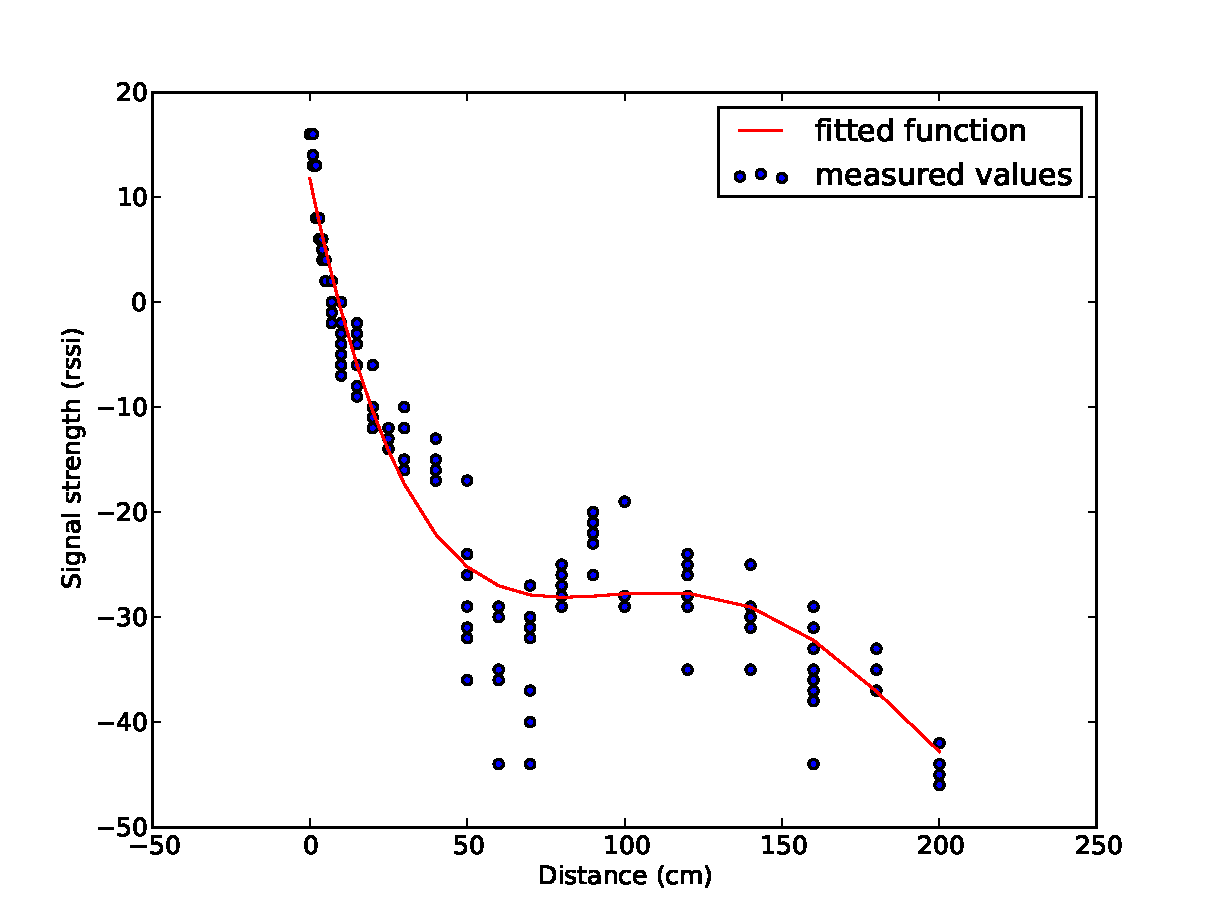
\includegraphics[width=\textwidth]{dataplot.pdf}
  \end{figure}
  The resulting 4th degree function is as follows.
  $$D = 1.64581191 \times 10^{-7} x^4 - 9.53330296 \times 10^{-5} x^3  + 0.0183046719 x^2 - 1.43727619 x + 11.7808933$$

  $x$ is the measured RSSI value. This function is used throughout the rest of the project wherever we need to obtain a distance from a RSSI value. As explained before, this is a best estimate, and can be considered inaccurate, but somewhat near the truth. [language...]
  
\section{Combining data with Kalman filtering}
We now have two sources of data, accelerometers and wireless signal strength. Both of these sources are easy to use, but inaccurate. To be able to know our location more accurately, we will combine data from both sources. 
\chapter{Measuring accuracy}

  \section{Method}
  \section{Results}

\chapter{Conclusion}

\chapter{Further work}
- add compass/gyro 

\chapter{References}
location, location, location

\bibliographystyle{unsrt}
\bibliography{fin}
\end{document}